\chapter{Implementation}\label{chapter:implementation}
This chapter explains how to set up a unikernel enabled Kubernetes cluster with the required components. It also goes into detail of different implementation ideas that are also possible to extend this project or that were implemented by other parties. Implementation of the project consists of 4 parts:
\begin{enumerate}
\item Setting up the Kubernetes cluster
\item Implementing a custom pod deployer
\item Setting up the edge environments
\item Developing unikernel applications
\end{enumerate}


\section{Setting up the Kubernetes Cluster}
The cloud provider selected for this thesis is Leibniz-Rechenzentrum, LRZ. They are using the OpenStack \cite{openstack} interface to provide computing services for their customers. While developing on the cloud, microK8s was used for setting up local,short-lived single-node clusters. The testing was done on a Kubernetes cluster set up by following the official documentation on their website. In that case, there is a Kubernetes master deployed on a VM with 20 GB Disk , 9 GB RAM, 2 VCPUs and running Ubuntu-18.04. The Kubernetes version is v1.16.3, which is the latest release at the time of writing. A secondary node is used for scaling experiments with the configuration similar to the master but with 4.5 GB RAM. The master node has a public IP so that devices can connect to it without a VPN. The pod network add-on used by the cluster is Cilium \cite{cilium}, as it's also being used by MicroK8s.

Another approach was to use Google Kubernetes Engine for setting up managed clusters. While their interface is easier to work with, connecting to them through non-Google-controlled devices is much more harder. They either require a device that is authorised with the \textit{gcloud} command line interface or they require a service account key file to be distributed alongside the kubeconfig file. While the first option was not a problem when registering the development PC as an additional node, it is suboptimal to install and authorise gcloud on IoT devices. It is a big application with many additional dependencies such as OpenSSL, thus unsuitable for the resource-constrained end devices. The second approach is much more resource friendly but just as similar to first approach, It is a security vulnerability waiting to be exploited as misconfigured service accounts can be used to run arbitrary commands on GCP using users' budget.

For local development, Minikube was also used on some parts of the project. Minikube only allows single node clusters unlike microK8s, but It was possible to register additional local nodes through valid kubeconfig to Minikube.

\section{Custom Pod Deployer}
Virtual Kubelet\cite{virtual} is an open source project by Microsoft that provides a programmable kubelet API interface to developers. It was developed to run workloads on Container as a Service providers, such as Azure Container Instances. When started with a valid kubeconfig file, virtual kubelet registers itself as a node to the Kubernetes cluster and executes commands given from the cluster. It has a programmable backend, called provider, through a golang interface for developers to write custom deployment logic to their own infrastructure. In Azure's case, using Virtual-Kubelet, they are registering their Azure service as a node with almost unlimited capacity, as Azure Container Instances, in theory, can scale up large number of containers without any restriction from the underlying hardware. There are also third-party providers, e.g. AWS fargate or Nomad, to offload workload to their respective container services. Microsoft also uses this techology to connect it's Kubernetes service with it's Azure IoT Hub service.\cite{Chandra2019} They are deploying docker containers to their edge devices through the Kubernetes API. 

A single virtual kubelet instance is started with the following command:
Virtual kubelet is started with the following command:
\begin{code}[htpb]
  \centering
  \begin{tabular}{c}
    \begin{lstlisting}[language=python]
      ./virtual-kubelet --nodename $ID --provider unikernel \\
       --kubeconfig kubeconfig.yaml --labels $LABELS
      \end{lstlisting}
\end{tabular}
\caption{Command to run Virtual Kubelet}\label{lst:vkcommand}
\end{code}


In the command \textit{\$ID} is a random generated string to give as node name. As virtual-kubelet can work with different providers, name of the provider is also given as argument. The provider written for this thesis is called \textbf{unikernel} and will be explained more in detail. \textit{\$LABELS} set Kubernetes node labels and it plays a big role on identifying different edge devices, thus multiple labels can be given.

While developing with virtual kubelet a side product of that effort was the ability to simulate large scale clusters within a reasonable budget. That part is explained in the next section.
\subsection{Simulating Large Scale Clusters}
The working principle of virtual kubelet is shown in figure \ref{fig:vk}. As virtual-kubelet is only a binary, it can run in a docker container and that docker container can be deployed to the same Kubernetes cluster and it uses the internal kubeconfig file to register itself as a node. In either case, those containers can be scaled to add new nodes to the Kubernetes cluster without scaling up the underlying hardware node count. This creates a testbed for researchers to test new scheduling algorithms. As every node can be given a arbitrary resource value from outside, different resource optimization cases can be tested in an artificially created mega cluster. A pod deployed to a virtual node, does not need to run and can be shown as healthly when queried by the Kubernetes master. The only workload that needs to be run is the virtual-kubelet binary, which only takes 34.3 MB in an alpine image when compressed with golang strip flags and upx. A fairly powerful single node Kubernetes cluster can run hundreds of it , and the user will see a 100+ node cluster.

\begin{figure}[htpb]
  \centering
  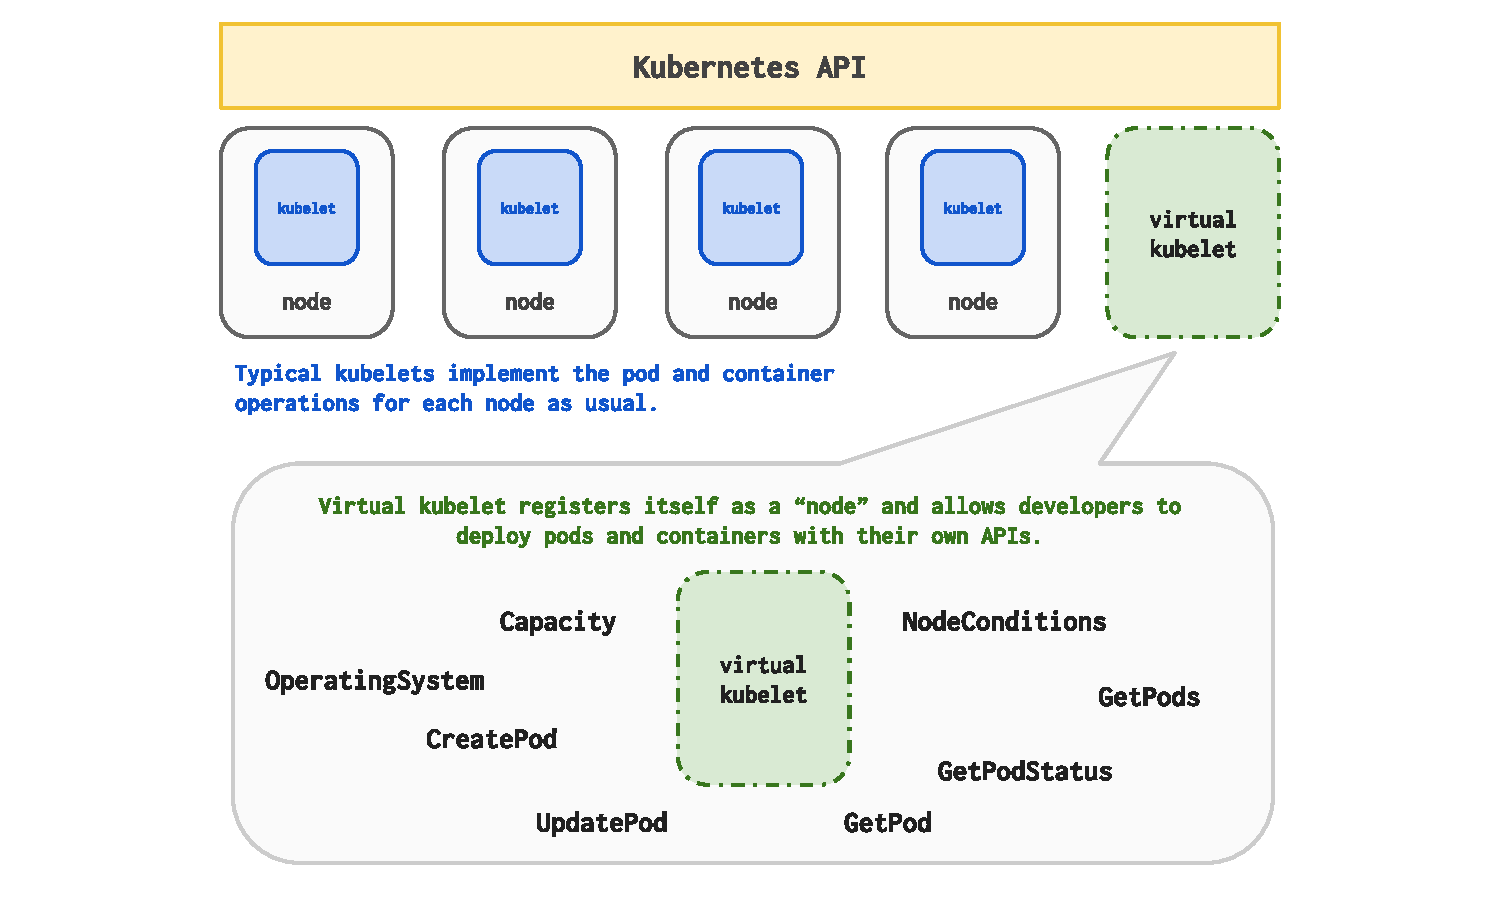
\includegraphics[width=1\textwidth]{figures/diagram.pdf}
  \caption{Working principle of Virtual Kubelet \cite{virtual}} \label{fig:vk}
\end{figure}

Another option is to run those containers in a different virtual machine , which is not a node of the target Kubernetes cluster. A valid kubeconfig can be used among running containers through a shared volume and a tool like docker-compose can be used to scale them. In this thesis, this approach was used for testing. A chunk of the docker-compose file can be seen in \ref{fig:docker-compose}.

\begin{code}[htpb]
  \centering
  \begin{tabular}{c}
  \begin{lstlisting}[language=ruby]
    services:
    node-temp:
      build: .
      image: atakanyenel/vk-client
      deploy:
        replicas: 2
      volumes:
        - ${PWD}:/tmp
      environment:
        - LABELS=sensor=temperature
\end{lstlisting}
\end{tabular}
\caption{A virtual node deployment}\label{fig:docker-compose}
\end{code}


A valid kubeconfig file can be found in the same directory as the docker-compose file and started containers use it to register themselves. When started, this configuration adds two additional nodes to the cluster with the label \textit{sensor=temperature}.

When creating virtual nodes, it's better to use docker containers , because virtual-kubelet binary listens on certain ports when running and it's hard to start two instances of it on the same machine. Docker containers provide that abstraction.

While testing for this thesis, edge devices were simulated on different virtual machines with different internet connections speeds. As it's impossible to test 100+ edge devices on the wild, nodes named Rpi-\{random-id\} were generated with different labels according to their simulated tasks.

\subsection{The Unikernel Provider}
The only customizable part of virtual-kubelet is the provider interface. The interface consists of 15 methods that needs to be implemented by the provider developer. Most of the methods are regarding the lifecycle of a pod, while some of them are responsible for the health of the node. 

This thesis implements a single provider called \textit{unikernel} for the unikernel runtime. A single virtual-kubelet binary can support multiple providers through command line arguments as can be seen from listing \ref{lst:vkcommand}. In this project, unikernel deployment is happening in 3 different environments. It's possible to write different providers for different environments but to decrease the built binary size,as all providers are built into the binary, a single provider was compiled using Golang's build tags for different environments. This requires the deployment medium to be known beforehand, instead of virtual-kubelet figuring it by itself by checking the installed hypervisor.

Current open source distribution of virtual-kubelet does not support giving labels to registered nodes. Label based scheduling is an easy way of deploying correct programs to edge devices, so virtual-kubelet source code had to be forked and modified to update node labels from outside with arguments.
\begin{code}[htpb]
  \centering
  \begin{tabular}{c}
  \begin{lstlisting}[language=python]
import "runtime"
(...)
var m runtime.MemStats
runtime.ReadMemStats(&m)
cpu := strconv.Itoa(runtime.NumCPU()),
memory := strconv.Itoa(int(m.Sys/1024/1024)) + "Mi"

\end{lstlisting}
\end{tabular}
\caption{Getting Resource data}\label{fig:runtime}
\end{code}
The first job done by the provider is to register the resources to the Kubernetes master as available. In the following code \ref{fig:runtime}, the provider constructor reads CPU and memory data from the device where virtual-kubelet is deployed. Kubernetes API uses standartised metrics for measuring CPU and memory, so read values are cast to string before being sent. There is also a third value called \textit{podCapacity}, which restricts the maximum number of pods that can be run on the device , independent from whether the device has enough resources or not.
% Golang Code block start

% Golang Code block end

\begin{code}[htpb]
  \centering
  \begin{tabular}{c}
  \begin{lstlisting}[language=ruby]
    func (s *Provider) DeletePod(ctx context.Context, pod *v1.Pod) error
\end{lstlisting}
\end{tabular}
\caption{DeletePod function Signature}\label{fig:signature}
\end{code}

The following list explains how other functions were implemented in unikernel and hypervisor context. All the functions have a signature similar to DeletePod function in figure \ref{fig:signature}.
\begin{description}
  \item  [Constructor] runs once and registers the node to cluster. It reads values with code block in \ref{fig:runtime}.
  \item [CreatePod] creates a pod with given pod information from the deployment yaml. All values can be read within the pod object. It calls an \textit{Execute} method, which runs the shell command to invoke the hypervisor with given parameters and returns the context information of the command. This information is saved to an in-memory map with pod name for further reference.
  \item [UpdatePod] updates the unikernel context in memory but not the running process. It's not possible to change parameters of running machines in Xen until next restart, so processes keep running instead of restarting them.
  \item [DeletePod] calls \textit{xl destroy <pod-name>} command to destroy the running unikernel. If the process is not a unikernel and a normal binary, it invokes the \textit{cancel} command which is saved with pod metadata.
  \item [GetPod] returns metadata about the pod from the in-memory map.
  \item [GetPodStatus] calls \textit{GetPod} and returns the status section from metadata.
  \item [GetPods] calls \textit{xl list -l} to get current hypervisor info and parses the json output, updates the in-memory map and returns it.
  \item [GetContainerLogs] find the command context from the map and returns it's stdout pipe. 
  \item [RunInContainer] is no-op.
  \item [nodeAddresses] is no-op but it's possible to return an IPv6 address in the future.
  \item [nodeDaemonEndpoints] returns a default value.
  \item [notifyPods] is no-op.
  \item [capacity] returns values set up with \ref{fig:runtime}.
  \item [ConfigureNode] is only called once. It's set up node information such as the running operating system, processor architecture, addresses...\ldots
  \item [nodeConditions] is called periodically to check on node. By checking the remaining capacity on the node, it might return one of the errors: \textit{OutofDisk}, \textit{MemoryPressure}, \textit{DiskPressure}, \textit{NetworkUnavailable}. Because this code is running periodically, developer can write custom functions to check their device for the mentioned errors.
  \end{description}
\subsection{Communication between cluster and device}
Once a virtual node is deployed to the cluster, it is crucial to restrict it to deployments it's supposed to handle. To achieve this, deployments regarding the virtual kubelet are tagged with a special label. First the \textit{nodeSelector} array of the specification get the item \textit{type: virtual-kubelet}. With that annotation , no real node tries to handle the deployment. The second annotation is to get the correct provider. In theory, a cluster can have multiple virtual nodes with different providers suited for different workloads and a deployment has to go to it's respective provider. Adding a \textit{tolerations} flag allows to select a particular provider. A chunk of an example deployment file can be seen in \ref{fig:deployment}.

\begin{code}[htpb]
  \centering
  \begin{tabular}{c}
  \begin{lstlisting}[language=python]
    (...)
    nodeSelector:
      type: virtual-kubelet
    tolerations:
    - key: "virtual-kubelet.io/provider"
      operator: "Equal"
      value: "unikernel"
      effect: "NoSchedule"
\end{lstlisting}
\end{tabular}
\caption{Node specific Deployment}\label{fig:deployment}
\end{code}
\textit{NoSchedule} effect protects real deployments from being handled by a virtual node. A pod without the exact tolerations will not be deployed to the node. It's easy to see that all that annotations work both ways. To isolate normal docker based deployments from virtual nodes and to isolate unikernel based deployments from real nodes.

Another approach of working with unikernel specific deployments is to extend the Kubernetes API by defining a \textit{custom resource}. Custom resources are more handcrafted, because they only contain information given by the developer. Stated by the Kubernetes API, "When you combine a custom resource with a custom controller, custom resources provide a true declarative API." Kubernetes has an Operator Pattern to extend the API in a more official way. In the first development iteration of the Operator Pattern, it turned out that the custom controller would only read data from the \textit{unikernel custom resource} and create a deployment configuration with the keys explained above and the information from the custom resource. Then, that deployment would be handled exactly the same, so it only saves the user from adding above mentioned keys but increases the complexity of the cluster greatly by adding a custom resource definition and a controller.

\subsection{Communication between virtual-kubelet and hypervisor}
Once a unikernel specific deployment reaches virtual-kubelet, all of it's data can be read. Every method that handles the pod lifecycle has a pod object as argument. This was already mentioned in  figure \ref{fig:signature}. The usability of this interface increases greatly when one realises that , this pod related information is not read or processed anywhere else other than the running node. It allows to redefine what those values stand for without comprimising integrity of the system. In a valid pod deployment, the \textit{image} key is used to specify the name of the docker container that deployment runs. If that container is not found in the given registry, Kubernetes returns an error saying that deployment failed and image couldn't be found. In the unikernel deployment, the image key is used to specify the name of the unikernel binary to run. That name can be handled in many ways. In earlier developments, docker containers simulating edge devices weree created with multiple example unikernel binaries, and there were only couple of options to give to \textit{image} key. Now a unikernel registry exists behind a FTP server and given values are searched there first, if they don't exist on the edge device. This approach is similar to one used by docker based deployments.

\textit{CreatePod} method is responsible for creating new pods. Upon receiving a new pod and checking that pod is valid, this  executes a shell command to talk with the underlying hardware. The shell command executes domain specific command with supplied parameters. The command runs in a subroutine, and status of the pod is updated as running. While specific commands will be explained more in the upcoming section, an interesting takeaway of this section is how the system does context management with those commands. These commands are all now running, and if they end up stopping for a reason, they have to be restarted by Kubernetes. \textit{GetPods} method is periodically called by the Kubernetes api and that method calls another shell command to check started unikernels. That output is then parsed as a pod object and returned back to master. The pods are saved in a dictionary with their name as key, and the context of their respective command as value. Their command context allows the system to call the \textit{cancel} closure of a command if that pod needs to be deleted, or their command output is send to the \textit{GetLogs} command to return command output. Golang is very helpful in that area ,because by design it has great mechanics for context aware concurrency.

\textit{nodeConditions} is also a periodically called function by the master and it can be configured to reflect changes on the host system. For example, if many unikernel images are running on device, there might be not enough memory to start more instances and that methods would change \textit{OutOfDisk} condition to true.

When a node disconnects from the Kubernetes cluster, Kubernetes does not re-deploy pods running on it until 5 minutes. The node shows up as NotReady but the pods are still running on it. This is an unwanted scenario for this use case, thus an additional container is deployed to the cluster to delete nodes when they disconnect. That deployment is called \textit{nodeWatcher}. It listens for events regarding nodes, and when a node disconnects, which has the \textit{virtual-kubelet} label, they are also deleted from the cluster. This allows cluster to redeploy pods running on the node without any delay. \textit{NodeWatcher} is a simple container written in python, without any complex logic. It can be used in other scenarios where rapid reaction to node disconnections are necessary.
\pagebreak
\section{Setting up end devices}
Unikernels, similar to traditional OS's can be booted directly from BIOS to hardware. Nevertheless, this is not flexible enough for cloud computing standarts, so hypervisors are used for on demand provisioning of unikernels. For proof of concept development, many different end device configurations were used. There are two different usage scenarios in mind when configuring devices. First one is hypervisor enabled unikernel runtime and the other one is with IoT.

For hypervisor-enabled runtime, a laptop was used. Installing a hypervisor on conventional virtual machines in the cloud was not possible because it breaks internal networking and makes it impossible to access machines from outside. Although it would be possible for different cloud providers, it's not a good testing environment as accessing to BIOS of a cloud provided virtual machine is not possible.

The mentioned laptop has Debian as the host operating system and Xen was installed through Debian with administrative priviledges to access BIOS. After Xen is installed, when laptop is booted up, user can select to start debian with Xen enabled. It's the same interface that a user sees when dual boots e.g. Windows or Linux. Starting with Xen gives xen daemon access to manipulate hardware. Because a linux system is installed on the computer that communicates with the hypervisor, it's a straightforward process to write Kubernetes clients. That laptop is connected to Kubernetes cluster through a valid kubeconfig file. Figure \ref{fig:hypervisor} shows the final overview of the setup. The virtual-kubelet runs on debian and communicates with Xen trough xen-cli, \textbf{xl}. Two additional linux VM's are traditional Kubernetes nodes connected with kubelet and they are running on the LRZ cloud.

\begin{figure}[htpb]
  
  \centering
  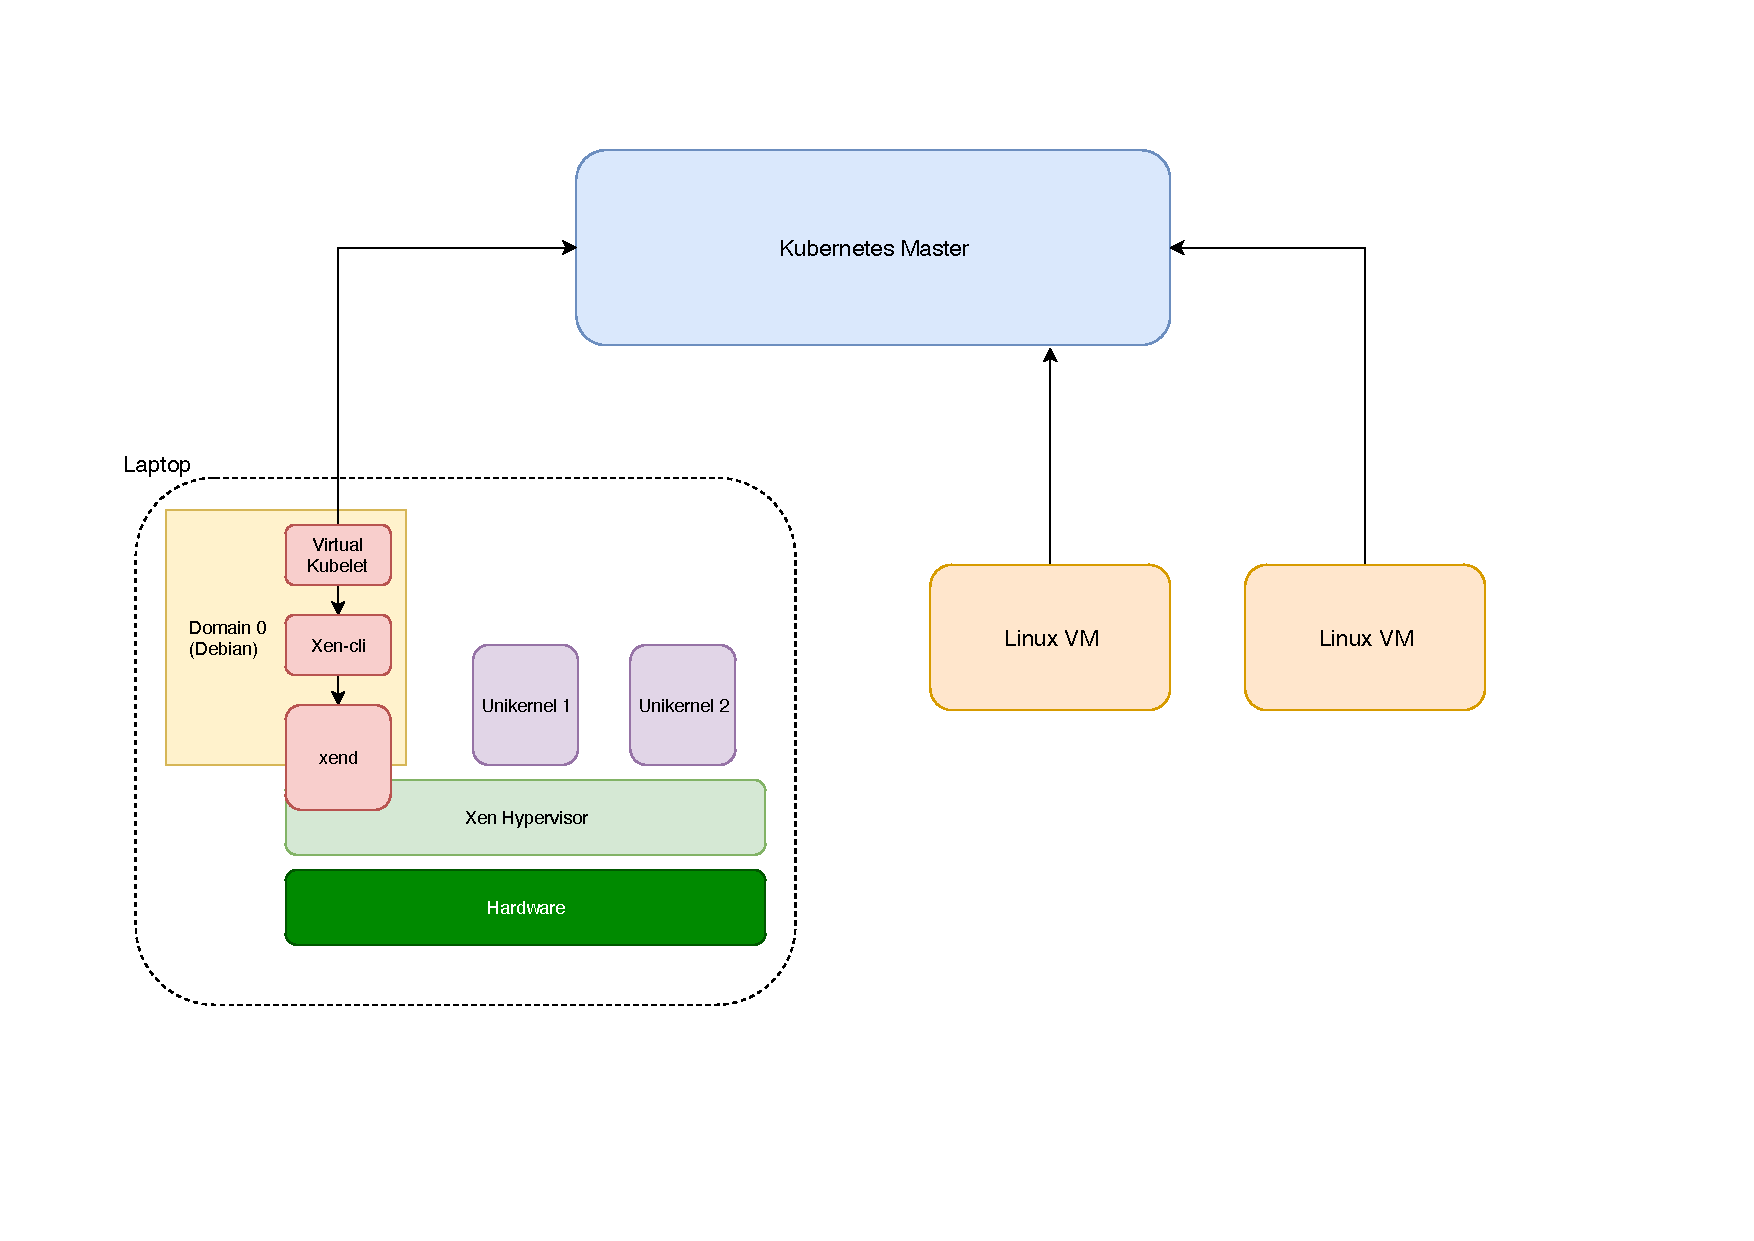
\includegraphics[width=1.2\textwidth]{figures/arch_new.pdf}
  \caption{ Kubernetes cluster with a only hypervisor enabled node for unikernel deployment} \label{fig:hypervisor}
\end{figure}


For further testing, a VM with Docker runtime was created. This VM does not have a kubelet and runs only virtual-kubelet to communicate with the Kubernetes cluster. It still runs Docker containers. The provider for that case was called \textit{Docker}. It was just for exercising the virtual-kubelet API and is not part of the final setup.

To experiment more with unikernel ecosystem, solo5 was installed alongside Xen to the aforementioned laptop. Solo5 can be built on top of Qemu or KVM and it markets itself as a unikernel specific runtime. To test Solo5, Qemu was installed because the hardware didn't allow KVM virtualisation.

Another enviroment is Docker containers running virtual-kubelet. They are built on top Ubuntu base image and unikernels can run on them. They are being used to simulate hundreds of IoT machines, since both Docker and Raspberry Pi lack hypervisor technology.

When configuring end devices for hypervisors, a network interface for unikernels should be set. If a unikernel application is using networking, the network interface should be given to the boot up command to make the local DHCP give it an IP.


For IoT devices, Raspberry Pi 3 was used. Raspberry Pi uses ARM processor and AMD64 hypervisors can't be ported easily. There is also not too much motivation for it, because Raspberry Pi is not a powerful end-device and not many virtualisation can be done on it. Despite that, there are projects for lightweight virtualisation on Raspberry Pi. For more powerful end devices though, there are hypervisor projects but they are out of scope for this thesis.

Despite lack of virtualisation, it's possible to run unikernels on Raspberry Pi by selecting Unix as the compilation target. Virtual-kubelet can also be compiled to ARM architecture and only takes 31 MB. A test setup was created with the circuit in \ref{fig:rpi-diagram}.

\begin{figure}[htpb]
  \centering
  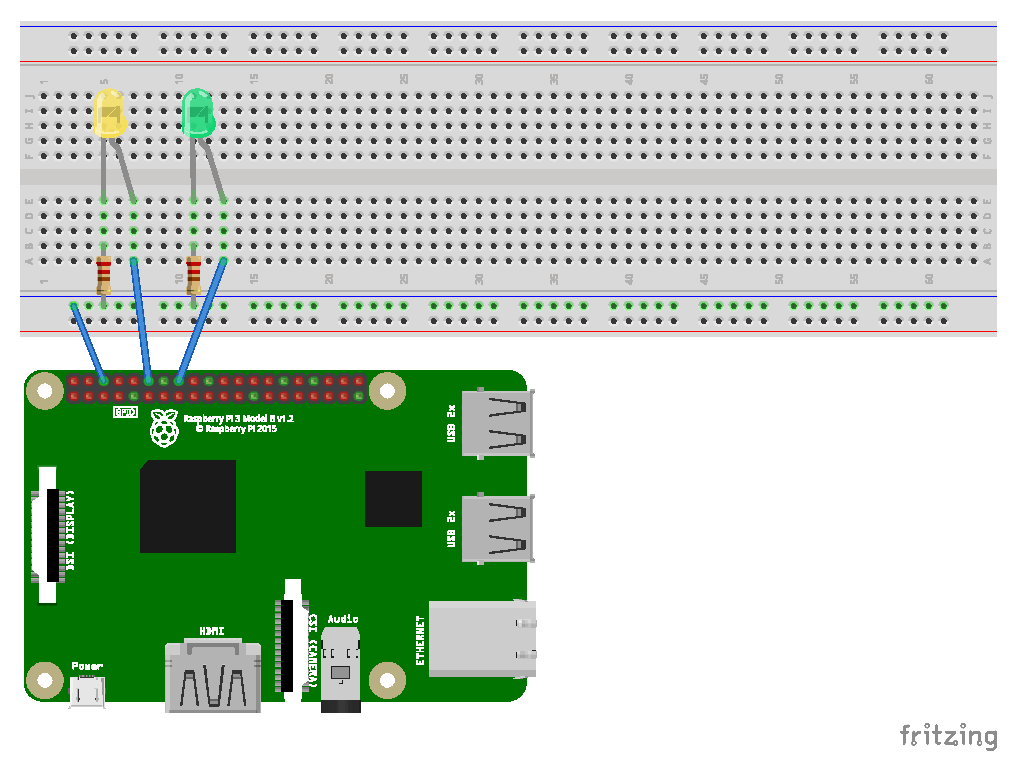
\includegraphics[height=0.6\textwidth]{figures/rpi-diagram.pdf}
  \caption{Yellow connected to pin 18 and green to pin 23} \label{fig:rpi-diagram}
\end{figure}

For the IoT case, two different DaemonSets are deployed to the cluster, namely yellow-daemon and green-daemon. Both DaemonSets are configured to deploy to nodes labeled with \textit{model=raspberry-pi}. While yellow-daemon is deployed to every node, green-daemon is only deployed to nodes if they have the \textit{light=GREEN} label additional to raspberry label. When a new device connects to cluster through virtual-kubelet, yellow-daemon deploys a unikernel application that turns the yellow led on. This workflow simulates the auto-configuration ability of this solution. The logic of the deployed application can be replaced with e.g. downloading additional binaries, sending GPS data only once, setting up a local network, etc.


When Raspberry Pi is labeled with \textit{light=GREEN}, green-daemon deploys another unikernel on the device, toggling green light on and off every 2 second. When the label is removed, virtual-kubelet kills the unikernel, which returns the green led to OFF state upon graceful termination. The unikernel applications get the pin number as a command-line argument. If a change occurs on the pin number that the led is connected to, the daemon can be edited on the fly with \textit{kubectl edit daemonset green-daemon} and the new pin number can be given to the \textbf{args} field. Termination of the unikernel with the outdated data and creation of the new one is handled completely by the Kubernetes API. The full YAML file for the mentioned DaemonSet can be seen in \ref{fig:green-daemon}.





\section{Developing Unikernel Applications}

Since Unikernel first introduced in 2013 by Madhavapeddy et al in \cite{library-operating-system}, there has been different language stacks to implement the proposed solution. Table \ref{tab:stacks} shows couple of state of the art projects with their target platform and their development language.

\begin{table}[htpb]
    \caption[Different Unikernel Stacks]{Different Unikernel Stacks}\label{tab:stacks}
    \centering
    \begin{tabular}{ |c |c |c| }
      \toprule
        Unikernel & Language & Target \\
      \midrule
        MirageOS & Ocaml & KVM,Xen, RTOS \\
        \hline
        OSv & Java,C,Node,Ruby & Virtualbox,KVM,Google Cloud, AWS,ESXi \\
        \hline
        HalVM & Haskell & Xen \\
      \hline
        Rumprun & C,C++, Erlang,... &  Xen, KVM \\
      \bottomrule
    \end{tabular}
  \end{table}

The reason for choosing MirageOS was the activity around its development and that it behaves directly as a unikernel. For example, both OSv and Rumprun have unused functionality on their kernels to support more languages.

MirageOS requires two files to develop a unikernel. First one is the \textit{config.ml} file. It defines the entry point of the program and lists dependencies. Second one is \textit{unikernel.ml} , which has the application entry point. To use a dependency, it has to be in the config file and adding a dependency requires additional files to be regenerated.

MirageOS uses an OPAM package with the name \textit{mirage} \cite{opammirage} for development. This package is used to create configuration files that will be sealed with the application code for the target environment and it also compiles the application. Drivers for unikernels are also written in Ocaml and published as additional opam packages. Once Mirage creates a deployment tree, it installs required packages through the OCaml repository. The following command in \ref{fig:mirage_configure} configures a package for compilation. 

\begin{code}[htpb]
    \centering
    \begin{tabular}{c}
    \begin{lstlisting}[language=bash]
      mirage configure --target hvt --kv_ro direct
  \end{lstlisting}
  \end{tabular}
  \caption{Generating unikernel specific files}\label{fig:mirage_configure}
\end{code}

That command targets the solo5 environment with \textit{hvt} value. \textit{kv\_ro} is a project specific flag, which tells unikernels to access the underlying file system directly to read key-value store.

After that step a \textit{Makefile} is generated for future commands. \textit{make depend} downloads dependencies for the program and \textit{make build} builds the unikernel. Build command compiles and seals the unikernel in couple of seconds, once the dependencies are installed. The build artifact is a single image. If it requires static files during build, they can either be packaged into the image or the image can be configured to access them during runtime.

\begin{figure}[htpb]
  \centering
  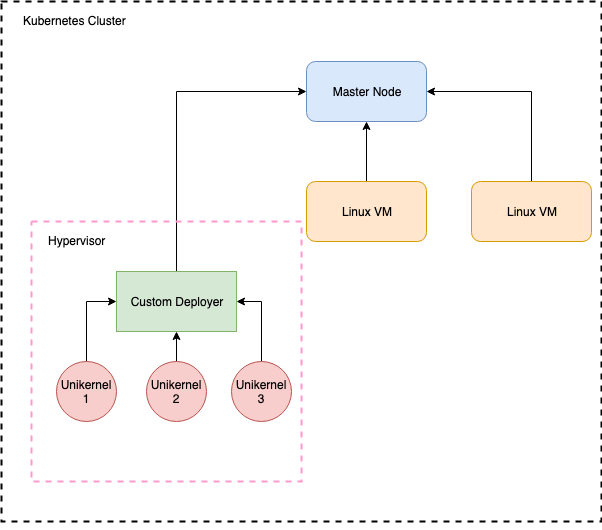
\includegraphics[width=0.8\textwidth]{figures/arch3.png}
  \caption{A Kubernetes cluster with a only hypervisor enabled node for unikernel deployment} \label{fig:hypervisor}
\end{figure}



\iffalse
\section{Proposed Solution}

Before starting to implement unikernels to Kubernetes, a couple of proof of concept unikernel programs will be created. To create those programs, open-sourced unikernel solutions will be used. There are multiple projects with different approaches and different runtime environments. Next chapter explains more about those solutions. Selecting the most suitable one for the purpose of this thesis plays a crucial role because, it is out of scope for this thesis to develop a new unikernel solution just for Kubernetes. Once those programs are created, unikernel deployments will be added to Kubernetes arsenal with the following steps:

1) A node with a type-2 hypervisor will be created. A custom program will be written that takes orders from a server and boot up unikernels according to parameters coming from the order. The custom program will run on the host operating system and there will be no Kubernetes involvement.

2) A Kubernetes cluster will be created and that custom program will be modified to communicate with Kubernetes. Everytime a unikernel deployment is made, Kubernetes will notify this program, and program will do the deployment.

3) Kubernetes DNS system will be integrated to the node with the type-2 hypervisor so they can communicate with other applications.

4) A node with a host operating system with type-1 hypervisor will be created. E.g. Xen hypervisor can also run on a host operating system. This node will be modified to communicate with the Kubernetes cluster through the host operating system. 

5) A node without a host operating system with type-1 hypervisor will be created. This node should also run the custom program that communicates with the Kubernetes cluster on the hypervisor and should also do the networking of unikernels between other Kubernetes resources.This will be the final outcome of the thesis.


A scope of this project is not to come up with a new unikernel solution and it will use the ones already developed by the open-source community.It also won't compare application performance between docker containers and unikernels. It will although compare the deployment time between those.
\fi